\section{Methodology}

In this section, we introduce \textbf{RLCER} (\textbf{R}einforcement \textbf{L}earning with \textbf{C}oT Supervision via Self-\textbf{E}volving \textbf{R}ubrics) for bootstrapping chain-of-thought reasoning. 
In the remainder of this section, we first briefly introduce the key idea of RLCER in Section \ref{sec:key-idea} to facilitate a high-level understanding. 
Then, we discuss the multiple roles under the same policy model in Section \ref{sec:roles}. 
After that, we discuss how to incentivize reasoning with self-proposed and rubrics in Section \ref{sec:reasoner_reward}. 
We then discuss how to self-evolve such rubrics in Section \ref{sec:reward_rubricator}.
Finally, we present how to optimize the policy $\pi_\theta$ under the two roles based on role-specific rewards in Section \ref{sec:policy-optimization}.

\subsection{Key Idea} \label{sec:key-idea}
\begin{wrapfigure}{r}{0.48\textwidth}
    \centering
    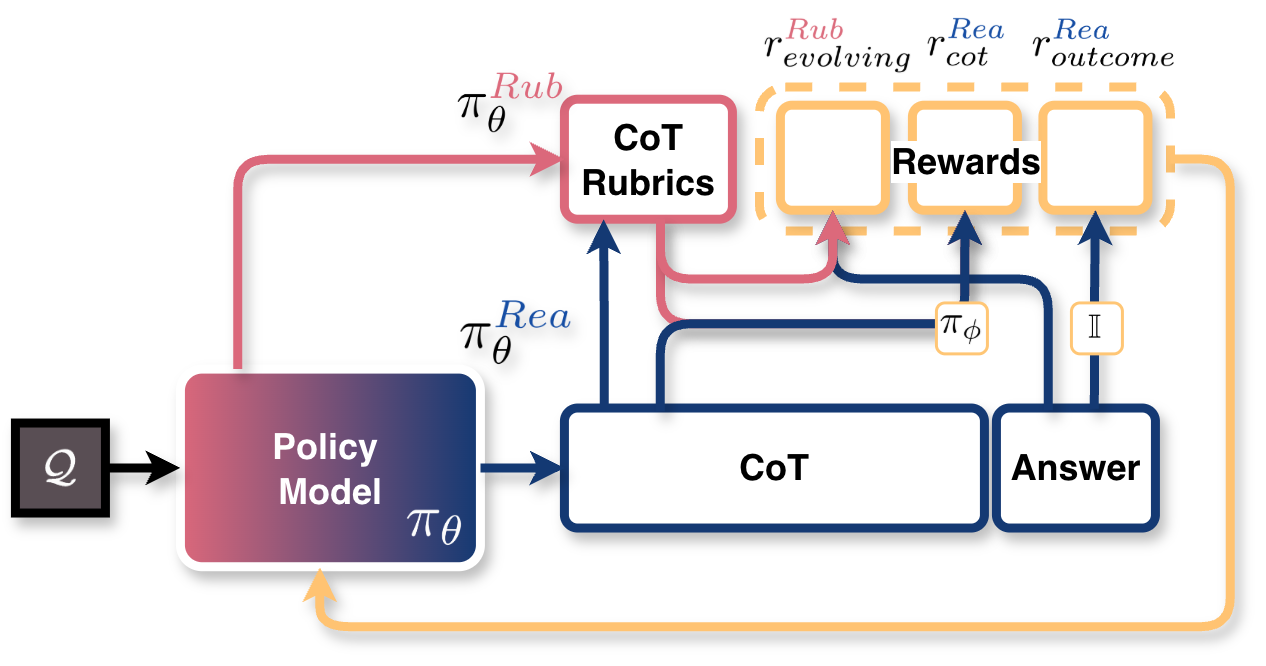
\includegraphics[width=\linewidth]{figures/framework/RLCER_key_idea.png}
    \vspace{-14pt}
    \caption{The RLCER loop. Format reward is ignored for brevity. One single policy model self-proposes rubrics for rewarding CoTs, and self-evolves the rubrics via rewarding generation capabilities.}
    \vspace{-8pt}
    \label{fig:key-idea}
\end{wrapfigure}

The key idea of RLCER is to go beyond rewarding what LLMs answer (\ie final-answer correctness) to explicitly and autonomously reward how LLMs think (\ie CoT quality) using self-proposed, self-evolving rubrics. The rubrics are evolved by tracking how well their satisfaction correlates with the final answer correctness.

To achieve this goal, we introduce two key roles in the multi-role RL framework for optimization: the reasoner $\pi_{\theta}^{\text{\textcolor{reasoner}{$Rea$}}}$ for answering the question and the rubricator $\pi_{\theta}^{\text{\textcolor{rubricator}{$Rub$}}}$ for generating rubrics supervising CoTs.
Here, the reasoner $\pi_{\theta}^{\text{\textcolor{reasoner}{$Rea$}}}(\cdot)=\pi_{\theta}(\cdot\mid\mathcal{P}^{\text{\textcolor{reasoner}{$Rea$}}})$ and the rubricator $\pi_{\theta}^{\text{\textcolor{rubricator}{$Rub$}}}(\cdot)=\pi_{\theta}(\cdot\mid\mathcal{P}^{\text{\textcolor{rubricator}{$Rub$}}})$ share the same policy parameter $\theta$, while their roles are distinguished by different prompts $\mathcal{P}^{\text{\textcolor{reasoner}{$Rea$}}}$ and $\mathcal{P}^{\text{\textcolor{rubricator}{$Rub$}}}$ respectively. 
The prompts can be found in Appendix \ref{apdx:prompts}. 
Additionally, a verifier $\pi_\phi$ is used for judging the satisfaction of rubrics, which is another fine-tuned and frozen model parameterized by $\phi$. 

As shown in Figure \ref{fig:key-idea}, we explicitly refine how the reasoner $\pi_{\theta}^{\text{\textcolor{reasoner}{$Rea$}}}$ thinks, by rewarding the CoT quality beyond the answer correctness, with the CoT quality evaluated by the verifier $\pi_\phi$ based on rubrics generated by the rubricator. 
We further enable rubric generation to self-evolve for more autonomous and effective CoT supervision by rewarding the quality of generated rubrics, guided by the correlation between rubric satisfaction degree and answer correctness.
We jointly optimize the policy model $\pi_\theta$ under two roles by assigning different rewards for each role. 
After computing role-specific rewards, we optimize the shared policy model $\pi_\theta$ for both roles, with advantages computed separately for each role \cite{SPICE}.


\subsection{Two Roles in One Policy: Reasoner and Rubricator} \label{sec:roles}
In this section, we take a closer look at the different roles of the reasoner $\pi_{\theta}^{\text{\textcolor{reasoner}{$Rea$}}}$ and the rubricator $\pi_{\theta}^{\text{\textcolor{rubricator}{$Rub$}}}$, within the RLCER framework.

\textbf{Reasoner} $\pi_{\theta}^{\text{\textcolor{reasoner}{$Rea$}}}$. 
The reasoner answers the question by generating a CoT $\hat{\mathcal C}$ and a final answer $\hat{\mathcal A}$.
Given the question $\mathcal Q$, the rollout sampling process of the reasoner can be formulated as:
\begin{equation}
\hat{\mathcal C}, \hat{\mathcal A} \sim 
\pi_{\theta}^{\text{\textcolor{reasoner}{$Rea$}}}\!\big(\cdot \mid \mathcal Q\big),
\end{equation}
where $\hat{\mathcal C}$ denotes the CoT process, and $\hat{\mathcal A}$ denotes the predicted final answer.

\textbf{Rubricator} $\pi_{\theta}^{\text{\textcolor{rubricator}{$Rub$}}}$.
The rubricator generates a set of $K$ rubrics for evaluating the CoT qualities based on the question $\mathcal Q$ and one CoT $\hat{\mathcal C}$. 
Given the question $\mathcal Q$ and a generated CoT $\hat{\mathcal C}$, the rollout sampling process of the rubricator can be formulated as:
\begin{equation}
\hat{\mathcal R} \sim 
\pi_{\theta}^{\text{\textcolor{rubricator}{$Rub$}}}
\big(\cdot \mid \mathcal Q, \hat{\mathcal C}\big),
\qquad
\hat{\mathcal R} \triangleq \{\hat{\tau}_k\}_{k=1}^{K},
\ \hat{\tau}_k \triangleq (\hat c_k,\hat s_k).
\end{equation}
The generated textual output $\hat{\mathcal R}$ contains $K$ specific rubrics, each denoted as $\hat{\tau}_k$. Here, $\hat c_k$ is the textual criterion (\eg ``avoids tangential explorations post-interval validation (3-$\infty$) by focusing on count aggregation'') of rubric $\hat{\tau}_k$ and $\hat s_k \in \mathbb{R}$ is the score of rubric $\hat{\tau}_k$ reflecting its importance, which can be both positive or negative. 
The rubrics generated under the rubricator role will then be used for judging the CoT quality through an external verifier $\pi_\phi$.

\subsection{Rewarding How to Think via Self-Proposed Rubrics} \label{sec:reasoner_reward}
In this section, we discuss how to autonomously reward how LLMs think via self-proposed rubrics. 

\textbf{Rewarding CoT with self-proposed rubrics.} Specifically, we reward a CoT based on how well it satisfies the valid rubrics proposed by the rubricator $\pi_{\theta}^{\text{\textcolor{rubricator}{$Rub$}}}$.
The CoT reward is computed by aggregating the scores of the satisfied rubrics:
\begin{equation}
    r_{cot}^{\text{\textcolor{reasoner}{$Rea$}}}=\texttt{norm}\left(\sum_{\hat{\tau}_{k} \in \hat{\mathcal{R}}_{valid}}\pi_\phi \left(\hat c_k, \hat{\mathcal{C}}\right)\cdot\hat s_k\right),
\end{equation}

where $\hat{\mathcal{R}}_{valid}$ denotes the set of valid rubrics from the rubricator, $\pi_\phi(\hat c_k, \hat{\mathcal{C}})\in\{0,1\}$ is a binary value produced by the verifier $\pi_\phi$ indicating whether the CoT $\hat{\mathcal{C}}$ satisfies rubric $\hat c_k$, and $\texttt{norm}(\cdot)$ is a normalization function that maps the aggregated score to the interval $[0,1]$. The function $\texttt{norm}(\cdot)$ conducts the min–max normalization as $\texttt{norm}(x) = (x-\text{MinValue}) / (\text{MaxValue}-\text{MinValue})$, where MinValue and MaxValue denote the minimum and maximum aggregated rubric scores attainable under the valid rubrics $\hat{\mathcal{R}}_{valid}$, respectively.

\textbf{Valid rubrics}. Here, a rubric $\hat{\tau}_k$ is considered valid if it is informative as a rewarding criterion: 
(i) its satisfaction indicator $\mathbf v_k$ is positively correlated with final-answer correctness $\mathbf z$
across $N$ sampled rollouts of the same question $\mathcal Q$ (\ie $\mathtt{corr}(\mathbf v_k,\mathbf z)>\alpha$),
and (ii) it is discriminative across different CoTs and would not yield consistent satisfaction (\ie $\mathtt{std}(\mathbf v_k)>0$). 
We define $\mathbf v_k$ and $\mathbf z$ over these $N$ rollouts as:
\begin{equation}
\begin{aligned}
\mathbf v_k &\triangleq \Big[\pi_\phi(\hat c_k,\hat{\mathcal C}_0),\ldots,\pi_\phi(\hat c_k,\hat{\mathcal C}_N)\Big],\\
\mathbf z   &\triangleq \Big[\mathbb{I}(\mathcal A,\hat{\mathcal A}_0),\ldots,\mathbb{I}(\mathcal A,\hat{\mathcal A}_N)\Big].
\end{aligned}
\end{equation}

The intuition is that higher correlation implies that satisfying the rubric is consistently associated with correct final answers and can produce informative rewarding signals. Here $\alpha$ is set as 0.2 by default in our paper. 

\textbf{Outcome reward.} The CoT reward $r_{cot}^{\text{\textcolor{reasoner}{$Rea$}}}$ can be used as an auxiliary reward alongside the outcome reward $r^{\text{\textcolor{reasoner}{$Rea$}}}_{outcome}$, which is calculated as follows:
\begin{equation}\label{eq:outcome_reward}
r^{\text{\textcolor{reasoner}{$Rea$}}}_{outcome} =  
\begin{cases}
  1, & \texttt{is\_equiv}(\mathcal{A},\hat{\mathcal{A}})\\
  -1, & \text{Otherwise.}
\end{cases}
\end{equation}

Following DAPO \cite{DAPO}, we assign a binary outcome reward based on final answer correctness: $r^{\text{\textcolor{reasoner}{$Rea$}}}_{outcome}$=1 if the predicted answer $\hat{\mathcal{A}}$ is equivalent to the ground truth answer $\mathcal{A}$, and $r^{\text{\textcolor{reasoner}{$Rea$}}}_{outcome}$=-1 otherwise. 

\textbf{Total reward for reasoner.} Finally, the overall reward for the reasoner is the combination of the outcome reward and the CoT reward:

\begin{equation}
r^{\text{\textcolor{reasoner}{$Rea$}}} = 
    r^{\text{\textcolor{reasoner}{$Rea$}}}_{outcome} + r_{cot}^{\text{\textcolor{reasoner}{$Rea$}}}.
\end{equation}

Such a reward enables autonomously optimizing what LLMs answer and how LLMs think simultaneously. 

\subsection{Rubrics Self-Evolving for Better Supervision} \label{sec:reward_rubricator}
While the two-role design enables a single policy model to self-propose rubrics for CoT supervision, we argue that such rubrics may get saturated: once consistently satisfied by all rollouts, they lose discriminative power over CoT quality and no longer provide reward signals, as shown in Section \ref{sec:reasoner_reward}. 
Therefore, we further propose to self-evolve the rubric generation capability, so as to progressively produce more informative and challenging rubrics that mitigate saturation.

\textbf{Self-evolving with validity reward.} To achieve rubricator self-evolving, we reward the fraction of the number of valid rubrics among all generated rubrics as follows: 
\begin{equation}
r_{evolving}^{\text{\textcolor{rubricator}{$Rub$}}}=\frac{K_{\text{valid}}}{K},
\end{equation}

% \clearpage
where $K$ and $K_{\text{valid}} \triangleq |\{\hat{\tau}^{valid}_k\}|$ are the numbers of all generated rubrics and valid rubrics, respectively. 
Such rewards encourage the rubricator to generate more informative rubrics that are positively correlated with answer correctness (\ie $\mathtt{corr}(\mathbf v_k,\mathbf z)>\alpha$) and discriminative (\ie $\mathtt{std}(\mathbf v_k) > 0$), thereby preventing rubric saturation. 
This reward provides a simple way for evolving the quality of generated rubrics, by connecting the satisfaction of the rubrics with the final answer correctness.

\textbf{Format reward.} Additionally, to ensure the proposed rubrics can be stably parsed, we reward the rubricator with a format reward, rewarding the correct format as follows:

\begin{equation}
    r_{format}^{\text{\textcolor{rubricator}{$Rub$}}}=\begin{cases}
  1, & \text{The format is correct.}\\
  0, & \text{Otherwise.}
\end{cases}
\end{equation}

\textbf{Total reward for rubricator.} Finally, the total reward for the rubricator is calculated as the combination of the quality reward and the format reward:

\begin{equation}
   r^{\text{\textcolor{rubricator}{$Rub$}}} =  r_{evolving}^{\text{\textcolor{rubricator}{$Rub$}}} + r_{format}^{\text{\textcolor{rubricator}{$Rub$}}}.
\end{equation}

Such a reward design encourages the rubricator to continuously refine its proposed rubrics, consistently providing informative rewarding signals for CoT supervision.  

\begin{figure*}[t]
    \captionsetup{justification=raggedright,singlelinecheck=false}
    \centering
    \scalebox{1}[1]{%
        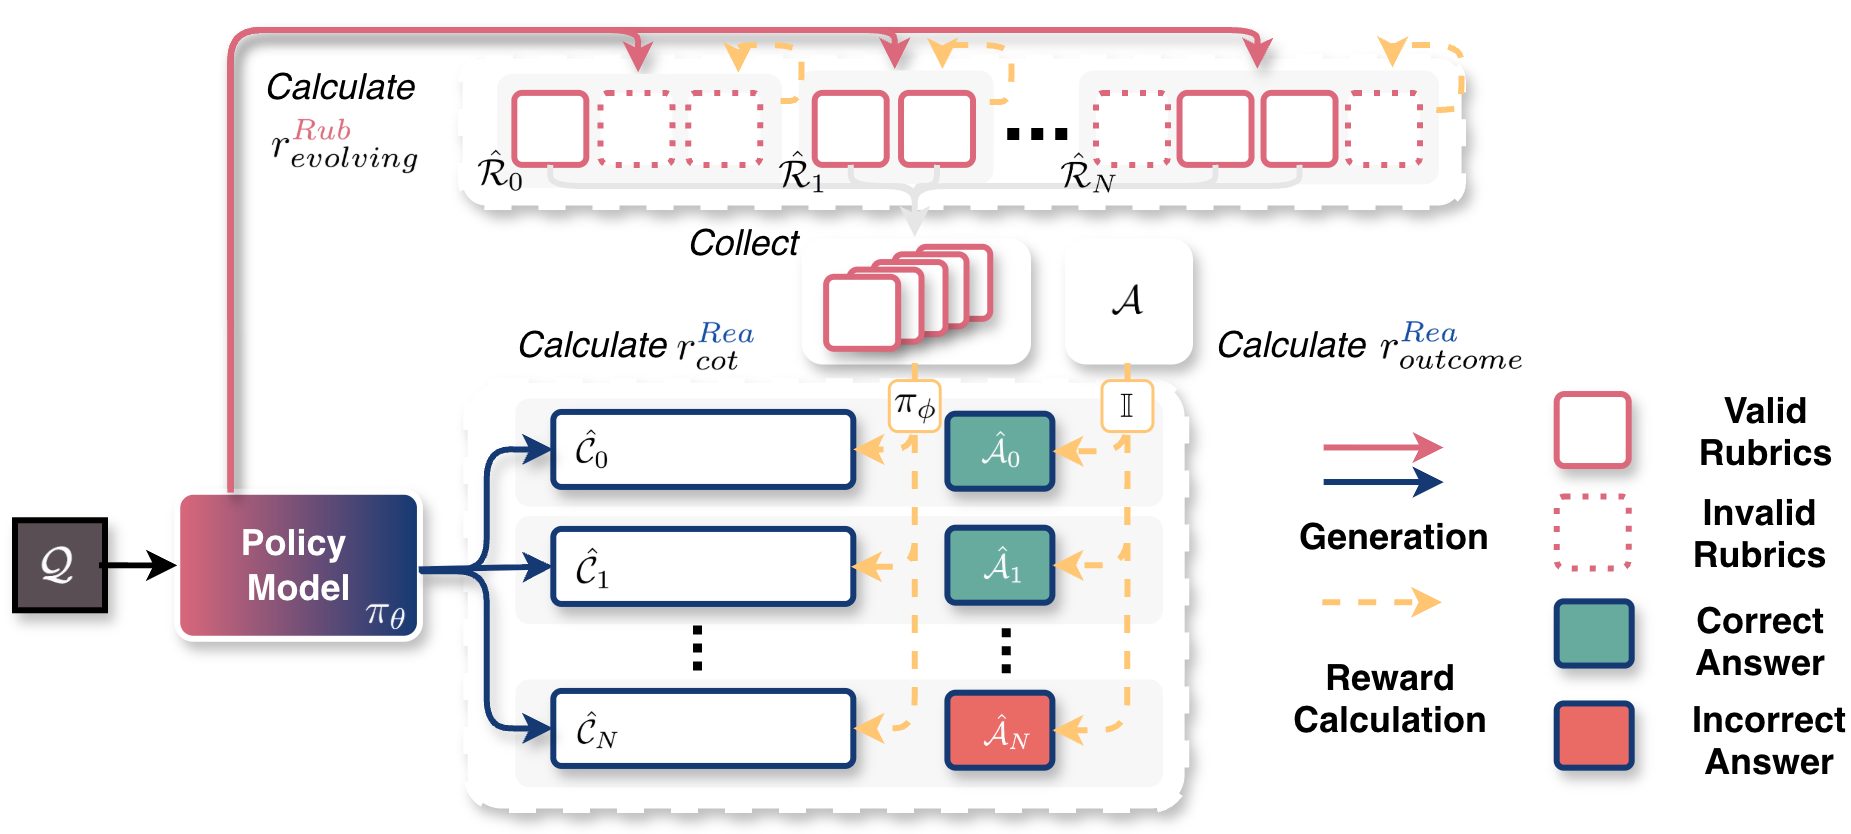
\includegraphics[width=0.88\textwidth]{figures/framework/RLCER_main_figure.png}%
    }
    \vspace{-6pt}
    \caption{Illustration of the reward calculation process in RLCER. For question $\mathcal{Q}$, the reasoner generates $N$ responses each with CoT $\hat{\mathcal{C}}_k$ and the final answer $\hat{\mathcal{A}}_k$. 
    After that, the rubricator generates $K_{n}$ specific rubrics (\ie $\hat{\mathcal R}_n \triangleq \{\hat{\tau}_k\}_{k=1}^{K_n}$). 
    The outcome reward is applied first by matching the generated answer $\hat{\mathcal{A}}_k$ with the ground-truth answer $\mathcal{A}$.
    All the valid rubrics (\ie $\mathtt{corr}(\mathbf v_k,\mathbf z)>\alpha$ and $\mathtt{std}(\mathbf v_k)>0$) are collected for rewarding CoTs. 
    And the fraction of valid rubrics for the $k$-th rubricator generation (\ie $\frac{|\{\hat{\tau}^{valid}_{n,k}\}|}{K_n}$) is used for rewarding the rubricator to self-evolve. 
    }
    \label{fig:main-figure}
    % \vspace{-6pt}
\end{figure*}


\subsection{Two-Role Optimization under a Single Policy} \label{sec:policy-optimization}

After computing the rewards for the reasoner and the rubricator, we jointly optimize the shared policy model $\pi_\theta$ under both roles in an end-to-end manner. Specifically, we compute role-specific advantages $\hat{A}^{\text{\textcolor{reasoner}{$Rea$}}}_t$ and $\hat{A}^{\text{\textcolor{rubricator}{$Rub$}}}_t$  from their respective rewards $r^{\text{\textcolor{reasoner}{$Rea$}}}$ and $r^{\text{\textcolor{rubricator}{$Rub$}}}$, and use them to update the policy via a standard policy-gradient objective. Gradients from both roles are aggregated to update the same set of parameters $\theta$, allowing the model to learn from role-specific feedback while maintaining a unified policy. The overall optimization procedure is illustrated in Algorithm~\ref{def:aglo}.

% \clearpage
With role-specific advantages $\hat{A}^{\text{\textcolor{reasoner}{$Rea$}}}_t$ and $\hat{A}^{\text{\textcolor{rubricator}{$Rub$}}}_t$, the optimization objective can be formulated as follows: 
\begin{equation}
\begin{aligned}
\mathcal{J}(\theta)
&= \ 
\mathbb{E}_{(\mathcal{Q}, \mathcal{A}) \sim \mathcal{D}^{\text{\textcolor{reasoner}{$Rea$}}},
\ \boldsymbol{o} \sim \pi^{\text{\textcolor{reasoner}{$Rea$}}}_{\theta_{\text{old}}}(\cdot \mid \mathcal{Q})}
\Big[
\min\Big(
\rho_t(\theta)\,\hat{A}^{\text{\textcolor{reasoner}{$Rea$}}}_t,\;
\text{clip}\big(
\rho_t(\theta),\,
1-\epsilon,\,
1+\epsilon
\big)\,\hat{A}^{\text{\textcolor{reasoner}{$Rea$}}}_t
\Big)
\Big],
\\
&+\mathbb{E}_{(\mathcal{Q}, \hat{\mathcal C}) \sim \mathcal{D}^{\text{\textcolor{rubricator}{$Rub$}}},
\ \boldsymbol{o} \sim \pi^{\text{\textcolor{rubricator}{$Rub$}}}_{\theta_{\text{old}}}(\cdot \mid \mathcal{Q, \hat{\mathcal C}})}
\Big[
\min\Big(
\rho_t(\theta)\,\hat{A}^{\text{\textcolor{rubricator}{$Rub$}}}_t,\;
\text{clip}\big(
\rho_t(\theta),\,
1-\epsilon,\,
1+\epsilon
\big)\,\hat{A}^{\text{\textcolor{rubricator}{$Rub$}}}_t
\Big)
\Big],
\end{aligned}
\end{equation}

where $\rho_t(\theta)$ is the policy likelihood ratio between $\pi_\theta$ and $\pi_{\theta_{\text{old}}}$ at step $t$, and $\epsilon$ is the clipping hyperparameter (\eg $0.2$). 
It is worth noting that GRPO is unsuitable for our algorithm, since the rubricator operates under different contexts, preventing its rollouts from being grouped under the same context required by GRPO \cite{DeepSeekMath}.


\begin{algorithm}[t]
\captionsetup{labelformat=default,labelsep=colon,name=Algorithm}
   \caption{Policy Optimization with RLCER}
   \label{def:aglo}
\begin{algorithmic}
   \STATE {\bfseries Input:} Question $\mathcal{Q}$, answer $\mathcal{A}$, the rollout sampling number $N$, and the maximum training steps $T$.
   \STATE {\bfseries Initialization:} initialize policy model $\pi_\theta$, training step $t \leftarrow 0$.
  \WHILE{$t \leq T$}
    % -------- Part 1: rollout (bg + label) --------
    \STATE \tikzmk{rlcerRolloutA} \CommentBelow{sample reasoner rollouts}
    \STATE $\{\hat{\mathcal{C}}_n, \hat{\mathcal{A}}_n\}_{n=1}^N \sim  \pi_{\theta}^{\text{\textcolor{reasoner}{$Rea$}}}(\cdot\mid\mathcal{Q})$
    \STATE \CommentBelow{sample rubricator rollouts}
    \STATE $\{\hat{\mathcal{R}}_n\}_{n=1}^N \sim  \pi_{\theta}^{\text{\textcolor{rubricator}{$Rub$}}}(\cdot\mid\mathcal{Q}, \hat{\mathcal{C}_n})$\tikzmk{rlcerRolloutB}
    % -------- Part 2: reward calculation (bg + label) --------
    \STATE \tikzmk{rlcerRewardA} \CommentBelow{calculate reasoner rewards}
    \STATE $\{r_n^{\text{\textcolor{reasoner}{$Rea$}}}\}_{n=1}^N =
    \{r^{\text{\textcolor{reasoner}{$Rea$}}}_{outcome,n} + r_{cot,n}^{\text{\textcolor{reasoner}{$Rea$}}}\}_{n=1}^N $
    \STATE \CommentBelow{calculate rubricator rewards}
    \STATE $\{r_n^{\text{\textcolor{rubricator}{$Rub$}}}\}_{n=1}^N =  \{r_{evolving,n}^{\text{\textcolor{rubricator}{$Rub$}}} + r_{format,n}^{\text{\textcolor{rubricator}{$Rub$}}}\}_{n=1}^N $\tikzmk{rlcerRewardB}
    % -------- Part 3: policy updating (bg + label) --------
    \STATE \tikzmk{rlcerPolicyA} \CommentBelow{calculate role-specifc advantages}
    \STATE Calculate $\hat{A}^{\text{\textcolor{reasoner}{$Rea$}}}_t$ and $\hat{A}^{\text{\textcolor{rubricator}{$Rub$}}}_t$
    \STATE \CommentBelow{policy optimization}
    \STATE Update policy $\pi_\theta$ via $\mathcal{J}(\theta)$\tikzmk{rlcerPolicyB}

    \STATE $t \leftarrow t+1$
   \ENDWHILE

   \STATE {\bfseries return} $\pi_\theta$.
\end{algorithmic}

% 画底色 + 右下角标签：放在 algorithmic 外面！
\boxit[Role-specific rollout]{RolloutBg}{rlcerRolloutA}{rlcerRolloutB}
\boxit[Rewarding]{RewardBg}{rlcerRewardA}{rlcerRewardB}
\boxit[Policy updating]{PolicyBg}{rlcerPolicyA}{rlcerPolicyB}
\end{algorithm}